\section{Architektura systému}
\label{sc:system_architecture}
Jak již bylo zmíněno v~nefunčních požadavcích, aplikace má být lehce rozšiřitelná. Tomuto požadavku se dá vyhovět několika způsoby, avšak ideologii Javascriptu se nejvíce blíží je modularizace \cite{bevacqua_2018_mastering}. A~pro lepší přehlednost kódu a zjednodušení testování samotných modulů, se jednotlivé moduly řídí metodikou \nameref{ss:clean_architecture}.

\subsection{Modularizace}
Aplikace byla modularizována tak, že nejprve byla rozdělena na jednotlivé domény, které je možné vidět na obrázku \ref{fig:class_diagram}. Následně tyto domény byly rozděleny na tři části, backend, frontend a společné.

\begin{figure}
    \centering
    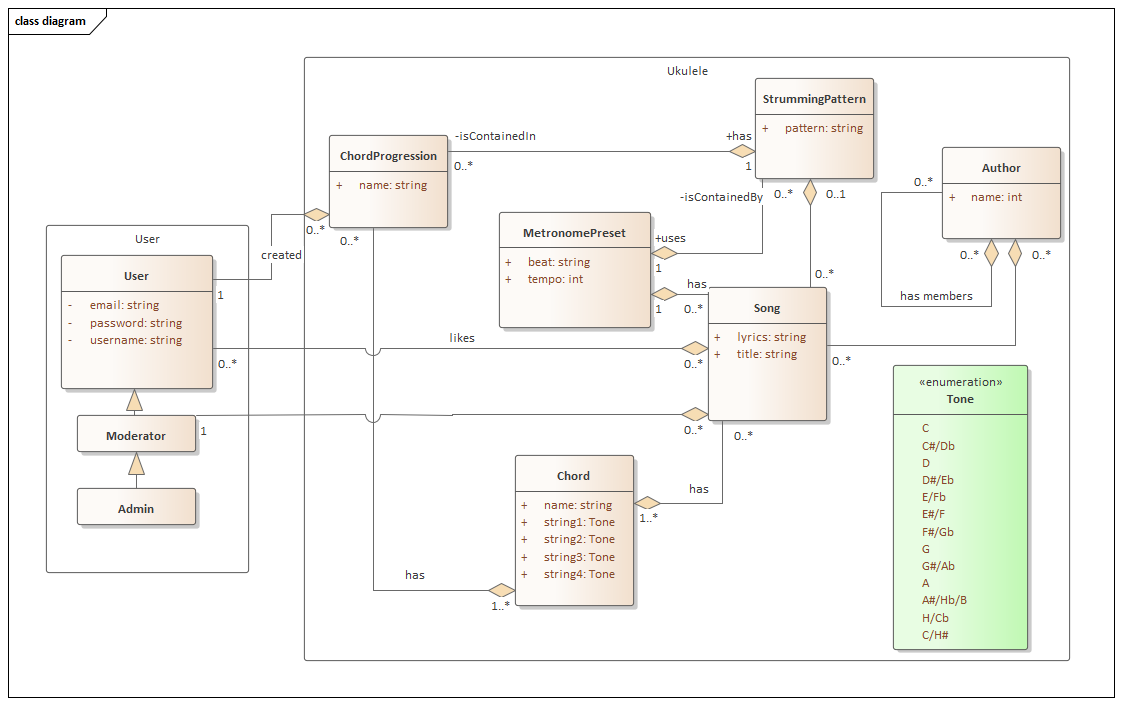
\includegraphics[width=\textwidth]{assets/class_diagram.png}
    \caption{Diagram tříd znázorňující dómény}
    \label{fig:class_diagram}
\end{figure}

Backend část specifikuje veškerou práci s~daty, která se odehrává na serveru, od validace až po vystavování mutací a query pro GraphQL server. Tato část smí být závislá jen na společné části domény a modulu autorizace. Díky tomu se zajistí striktní oddělení domén a zjednodušší testování, jelikož jednotkové testy pak testují jen skutečně jednu funkcionalitu nezávisle na všech ostatních. Každý takovýto balíček exportuje jednu funkci, která jako parametr dostane nastavení a vrací objekt obsahující \emph{seed} pro inicializaci aplikace, mutace a query pro GraphQL server.

V~části frontend jsou vytvořeny jednotlivé komponenty, zase pouze pro jednu danou doménu. Tato část je závislá pouze na společné části domény, na modulu autorizace a na modulu \emph{look}, který udává vzhled aplikaci, tím že obsahuje základní komponenty, jako například tlačitko nebo základní vstupní pole. Takovýto balíček exportuje dané komponenty.

Takto rozdělené části tvoří balíčky. Tyto balíčky na sobě závisí, tak jak bylo popsáno výše a tyto závislosti jsou spravovány právě pomocí \ref{ss:yarn} jako monorepo. Jednotlivé balíčky mají unifikované jména, a to takto:~\sloppy{\emph{uls@<doména>-<react|nodejs|common>}} kde uls je zkratka pro \emph{ukulele learning site}, což je pracovní název aplikace.

Jednotlivé balíčky ovšem netvoří výslednou aplikaci, proto je potřeba mít ještě další dva speciální balíčky, jeden pro backend a druhý pro frontend. Backend balíček importuje všechny inicializační funkce, vytvoří inicializační parametry, vytvoří jednotlivé moduly a následně je registruje do GraphQL serveru. Frontend balíček nejen, že importuje všechny komponenty, ale následně je skládá na stránky. Jednotlivé komponenty tedy neví, v~jakém kontextu a kde budou zobrazeny a proto je potřeba aby byly správně zapouzdřené a komunikovali jen pomocí vstupních parametrů. Top level balíček, ten který je nadřazený všem, vytváří pouze testovací prostředí a slouží jako root balíček pro všechny moduly tak, aby mohlo správně fungovat monorepo.


\begin{figure}
    \dirtree{%
        .1 root projektu.
        .2 modules\DTcomment{Adresář s~moduly}.
        .3 look\DTcomment{Modul udávající vzhled aplikace}.
        .4 react.
        .3 ukulele\DTcomment{Modul obsahující doménu hry na ukulele}.
        .4 common.
        .4 nodejs.
        .4 react.
        .3 \ldots .
        .2 packages.
        .3 nodejs\DTcomment{Sestavuje backend server}.
        .3 react\DTcomment{Sestavuje frontend server}.
    }
    \caption{Zjednodušená adresářová struktura}
    \label{fig:modules}
\end{figure}

\subsection{Clean Architecture}
\label{ss:clean_architecture}
Tato metodika, prezentovaná ve stejnojmené knize od R. C. Martina~\cite{martin_2018_clean}, popisuje jak rozdělit aplikaci na jednotlivé vrstvy. Říká, že aplikace by měla být rozdělena na \emph{entity}, \emph{use case}, \emph{presenters, controllers} a \emph{frameworks, drivers}, znázorňující obrázek \ref{fig:clean_architecture}.
Entity definují základní byznys pravidla dané domény a jejich reprezentace může být například sada funkcí, nebo objekt s~metodami nebo bez. V~rámci této práce jsou entity reprezentovány pomocí objektů bez metod, přesněji Typescript interfaces, a to hlavně z~důvodu snadné serializace a deserializace.
Vrstva use case provadí operace specifické pro aplikaci nad danými entitami. V~případě této práce to jsou \emph{intereactory}, třídy které manipulují s~entitami.
Následující vrstva už převádí dané entity na objekty vhodné pro další vrstvu frameworků, jedná se tedy o~interface. V~této práci je tato vrstva Mongoose modely, se kterýmy následně pracuje databáze a zároveň ze kterých se generuje GraphQL API, kterým backend předává informace frontendu. A~poslední vrstvou jsou samotné frameworky či databáze, v~případě této práce se jedná o~React, resp. MongoDB, které informace zobrazují, resp. ukládají.

Výhodou tohoto rozdělení je přehlednost a hlavně snadné testování. Při testování dané vrstvy, se vždy přistupuje z~vrstvy nadřazené, test tedy simuluje operace které by dělala vrstva nadřazená a mockuje se první podřazená vrstva. Je tedy vždy jasné jak daný test funguje a jaká data testuje. V~případe těchto testů mluvíme o~testech jednotkových, nikoliv smoke nebo integračních.

\begin{figure}
    \centering
    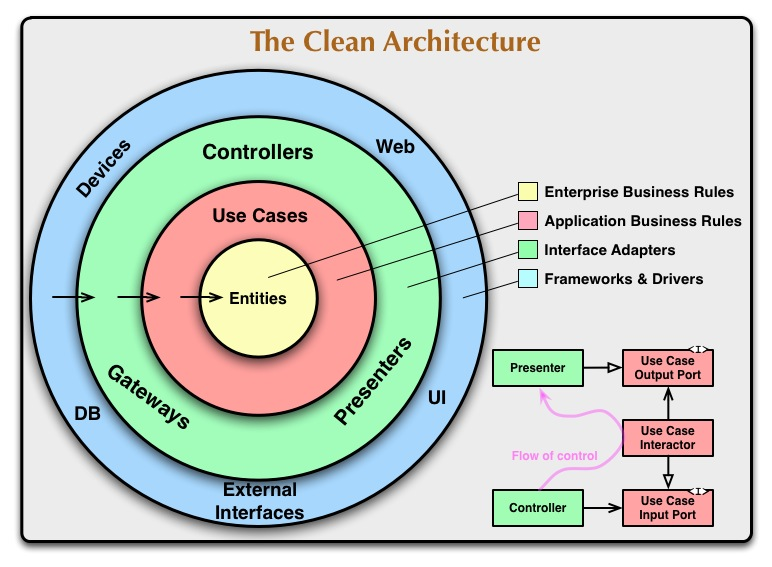
\includegraphics[width=\textwidth]{assets/clean_architecture.jpg}
    \caption{Clean Architecture}
    \label{fig:clean_architecture}
    \textit{Zdroj:}~https://blog.cleancoder.com/uncle-bob/2012/08/13/the-clean-architecture.html
\end{figure}
